\autsection{General Approach}{Nelián Colón}

Due to the nature of project, most of the work will be completed trough
developer workstations. At first, the team will be developing different parts of
the system as they are all loosely coupled. Test driven development will be
done, meaning that after each part gets successfully developed and united
tested, only then they are integrated and tested from a bigger perspective. The
project is divided into 4 major parts, these are: Front end Client, Back end
Server, Test Framework, and Repository Manager, as shown in Figure~\ref{arqu}.
The team will be using a single
cloud hosted Git repository (GitHub) where the project's code will live, and
will follow best revision control practices. Moreover the team will follow the
Scrum agile development process and will confine to good planning and
documentation.

\begin{figure}[H]
	\centering
	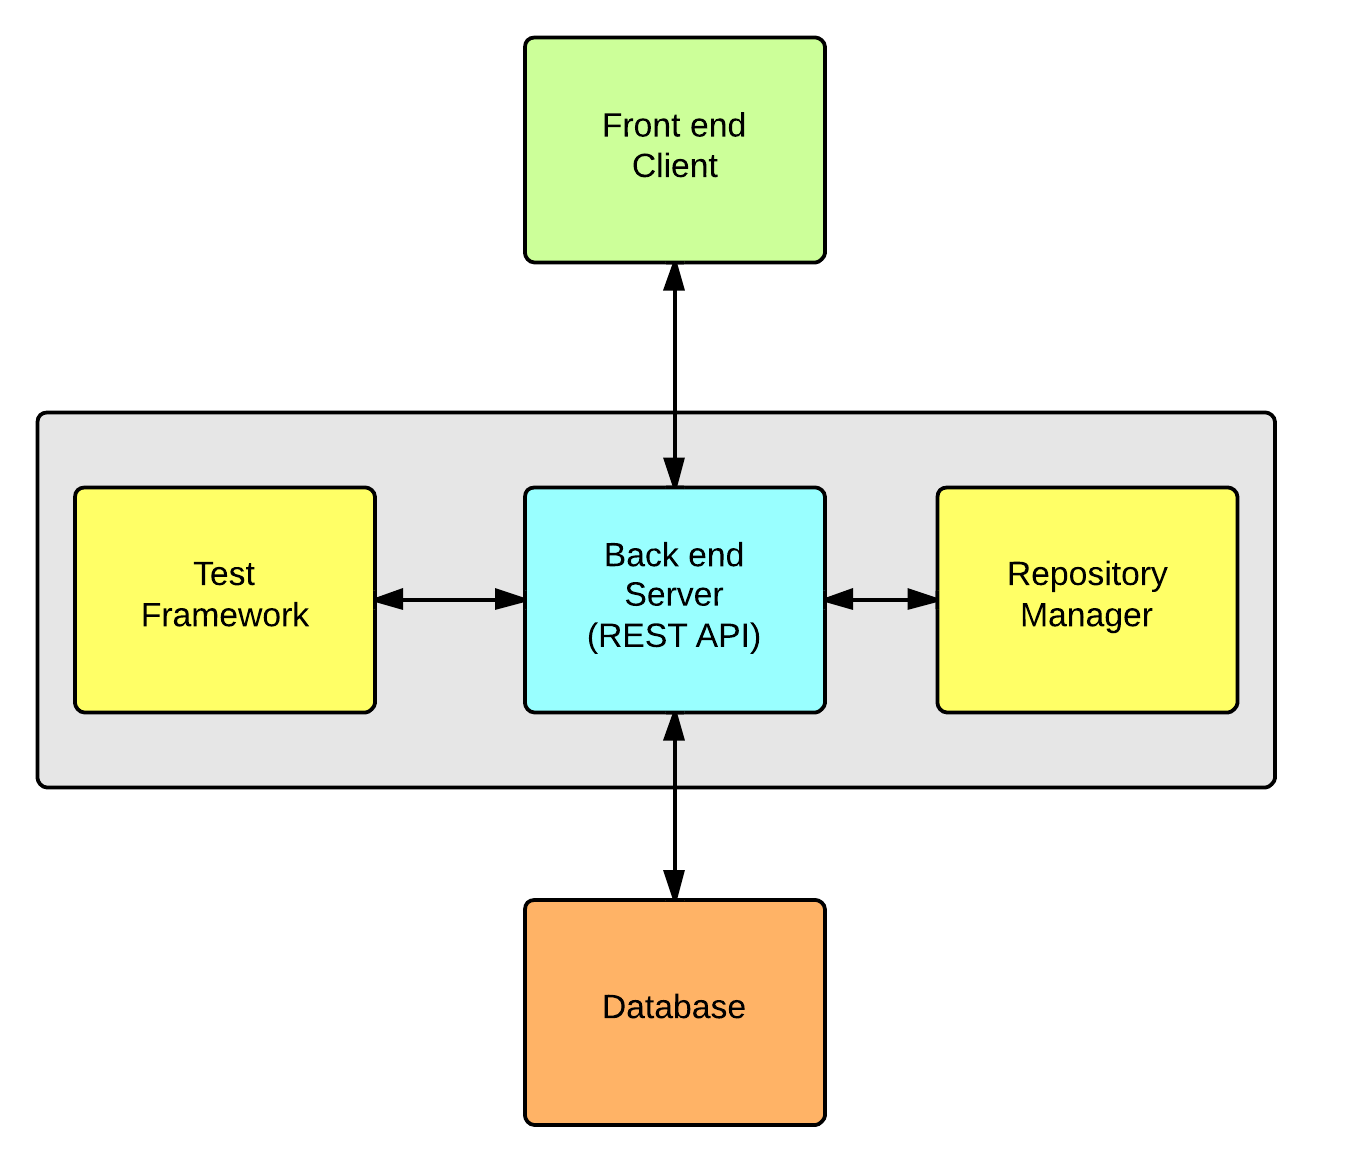
\includegraphics[width=\textwidth]{img/bigArquitectOverview}
	\caption{General overview of the system\label{arqu}}
\end{figure}

\subsection{Meetings and Work Hours}

Team Aguacate will hold weekly meetings on Tuesdays from 3:00 pm to 4:00 pm to
discuss progress and project details. In each meeting, each member will state
his/her progress, any needs he/she might have and if their schedule has changed.
Work hours on assigned tasks will occur every Monday, Wednesday, and Friday from
9:30 am to 11:20 am unless there is a seminar scheduled for that day. Other work
hours will be every possible day from 6:00 pm to 9:00 pm, minimum. The team will
work on sprints, so a sprint planning meeting will occur on Thursdays from 3:00
pm to 4:00 pm whenever a new sprint comes. Meeting agendas minutes will be
posted in our blog: \url{http://pandacodereview.wordpress.com/}.

\subsection{Team Management}

The meetings will be as described above and other meetings will be scheduled
when needed. One of the purposes of these meetings is to make sure that each
team member is aware of the other members' progress and concerns. Changes to
these hours are to be discussed and decisions will depend on majority vote and
team leader opinion. Each task will have a leader and an assistant. The leader
of each task is responsible for it and the assistant will assist whenever the
leader gets stuck on a problem. Whenever a conflict arises, the member involved
is responsible of looking for a mediator as soon as possible to help him/her
solve the problem.

\subsection{Documentation Standards}
See Appendix~\ref{sec:stand} to see documentation standards.
